\documentclass{article}
\usepackage{tikz}
\usetikzlibrary{arrows}
\begin{document}

\begin{figure}[h!]
    \centering
    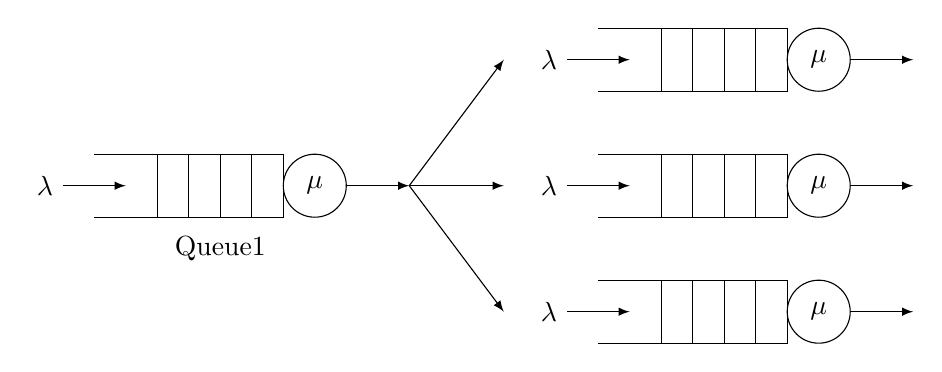
\begin{tikzpicture}[>=latex,scale=0.8]
    \foreach \x/\y in {0/0,8/2,8/0,8/-2}
      {
      \pgfmathsetmacro{\r}{0.5}
      \pgfmathsetmacro{\l}{3}
        \draw (\x-\r-\l,\y+\r) -- ++(\l,0) -- ++(0,-2*\r) -- ++(-\l,0);
        \foreach \i in {1,...,4}
            \draw (\x-\r-\i*0.5,\y+\r) -- +(0,-2*\r);
        \draw (\x,\y) circle (\r);
        \draw[<-] (\x-\l,\y) -- +(-2*\r,0) node[left] {$\lambda$};
        \draw[->] (\x+\r,\y) -- +(2*\r,0);
        \node at (\x,\y) {$\mu$};
      };
      \draw[->] (1.5,0) -- (3,2);
      \draw[->] (1.5,0) -- (3,0);
      \draw[->] (1.5,0) -- (3,-2);
    \node at (-1.5,-1) {Queue1};
\end{tikzpicture}
 \caption{Queue Network}\label{fig:queueNetwork}
\end{figure}

\end{document}
